% IEEE Access manuscript. Built on IEEEtran (journal mode) so that it compiles with a
% standard TeX Live installation; see README.md for moving the text into the
% official IEEE Access template (ieeeaccess.cls) before submission.
\documentclass[journal]{IEEEtran}
\usepackage{amsmath,amssymb}
\usepackage{graphicx}
\usepackage{booktabs}
\usepackage{array}
\usepackage{multirow}
\usepackage{cite}
\usepackage{url}
\usepackage{algorithm}
\usepackage{algpseudocode}
\usepackage[hidelinks]{hyperref}

\graphicspath{{figures/}}
\newcommand{\pu}{\,pu}
\newcommand{\todo}[1]{\textbf{[TODO: #1]}}
\newcolumntype{P}[1]{>{\raggedright\arraybackslash}p{#1}}
\algrenewcommand\algorithmicrequire{\textbf{Input:}}
\hyphenation{Grid-PACK HELICS syn-chro-pha-sor}

\begin{document}

\title{A Remotely Accessible GridPACK--NS-3--HELICS Testbed for Synchrophasor-Based Monitoring and Control Under Cyber Attacks}

\author{Md~Mazharul~Islam,
        Sunjare~Zulfiker,
        Masum~Reza,
        and~Hafiz~Abdur~Rahman%
\thanks{The authors are with the Department of Electrical and Computer Engineering, North South University, Dhaka 1229, Bangladesh (e-mail: mazharul.islam1@northsouth.edu; sunjare.zulfiker@northsouth.edu; masum.reza@northsouth.edu; hafiz.rahman@northsouth.edu).}%
\thanks{Corresponding author: Hafiz Abdur Rahman (e-mail: hafiz.rahman@northsouth.edu).}%
\thanks{This work was supported by the Bangladesh Energy and Power Research Council (EPRC) under grant EPRC/58-2018-007-01.}}

\markboth{IEEE Access}{Islam \MakeLowercase{\textit{et al.}}: A Remotely Accessible GridPACK--NS-3--HELICS Testbed}

\maketitle

\begin{abstract}
Phasor measurement units (PMUs) give control centers time-stamped phasors many times per second, but their value depends on the network that carries the frames and on whether the frames can be trusted. Hardware testbeds for this chain are costly and serve few users, while open-source co-simulations target distribution systems or omit the measurement chain and its defenses. This paper presents an open-source, remotely accessible testbed for the complete synchrophasor loop under network impairments and cyber attacks, and measures which parts of the loop decide whether an attack succeeds. GridPACK solves the power flow as a persistent message passing interface (MPI) job, NS-3 carries every PMU frame and command through a phasor data concentrator (PDC), and a control center performs state estimation, chi-square bad data detection with normalized-residual removal and voltage control. HELICS synchronizes the federates, and users work from a web dashboard. On the IEEE 118-bus system, 225 runs combined an automatic voltage regulator fault with four attacks, two PMU placements, five link latencies and five PDC wait windows, each with ten random seeds. With 32 PMUs, detection without removal, delay and drop each stretched the over-voltage from 0.5 to 5.5\,s in every seed, and with 68 PMUs no attack extended it. Without any attack, 40\,ms of mean link latency and a 20\,ms wait window hid the fault in six of ten seeds. Removing bad data, redundant placement and a wait window chosen from the delay spread therefore matter as much as the detection test.
\end{abstract}

\begin{IEEEkeywords}
Co-simulation, cyber-physical systems, false data injection, GridPACK, HELICS, NS-3, phasor data concentrator, phasor measurement unit, state estimation, testbed.
\end{IEEEkeywords}

\section{Introduction}
\label{sec:intro}

\IEEEPARstart{F}{or} decades, transmission control centers have watched the grid through supervisory control and data acquisition (SCADA). Remote terminal units report unsynchronized magnitudes every few seconds, and the state estimator needs iterations over a nonlinear model to turn them into bus voltages \cite{abur2004se}. A phasor measurement unit (PMU) changes this picture. It samples the voltage at its bus and the currents on the branches connected to it, stamps each frame with time from the global positioning system (GPS), and sends 30 to 60 frames per second to a phasor data concentrator (PDC) \cite{phadke2008,c37118_1}. The PDC aligns the frames by time stamp and passes sets to applications in the control center. Because the phasors are linear in the bus voltages, the control center can estimate the state in one step and act on it within a fraction of a second \cite{phadke2008,abur2004se}.

Two things limit what the control center can do with these data. The first is the communication network. A frame that arrives after the PDC has released its time stamp is lost for that set, and a set that misses PMUs can leave part of the grid unobserved \cite{c37244,pourramezan2021pdc}. The second is trust. An attacker who can change frames can try to hide a real problem or create a false one. Liu \emph{et al.} showed that an attacker who knows the measurement model can add an error that the residual test of the estimator cannot see \cite{liu2009fdi}, and later studies examined how many measurements such an attack needs, how to protect them and how to catch the attack with learned detectors \cite{kosut2011,bobba2010,chen2022datadriven,bhattacharjee2023deep}. Attacks on timing are just as effective. Shifting the time reference of a PMU or delaying its frames makes the PDC drop them \cite{zadsar2023preventing,shereen2024topology}.

These questions cross the boundary between the power system and the network, so studying them requires both to be simulated together, with the PMUs, the PDC and the control center in between. Real-time hardware testbeds do this with high fidelity \cite{kumar2025rtcptc,nguyen2024rtcps,das2025scalable,mishchenko2024multidomain}, but they cost a great deal, and the number of experiments they can run at once is fixed by the hardware. Open-source co-simulation platforms built on HELICS \cite{palmintier2017helics,hardy2024helics} lower the cost, yet the recent ones model distribution feeders, advanced metering or distributed energy resources \cite{bel2024natig,thioub2026gridsecsim,vallamkondu2025der,masood2026cosim}, or couple transmission and distribution without any network \cite{zheng2024hpc}. Our own earlier prototype coupled GridPACK and NS-3 on the IEEE 14-bus system and studied distributed denial of service (DDoS), but it had no PMU chain, no estimator and no closed loop \cite{islam2024remotely}. None of these platforms lets several users run transmission-level synchrophasor experiments from a browser on shared computing resources, and none reports, for one system and one fault, how the PDC wait window, the spread of link delays, the redundancy of PMU placement and the choice between detecting and removing bad data change the outcome of an attack.

This paper fills that gap with an open-source testbed and an experimental study on the IEEE 118-bus system. Its contributions are as follows.
\begin{enumerate}
\item A co-simulation of the complete synchrophasor loop in which GridPACK \cite{palmer2016gridpack} runs as a persistent message passing interface (MPI) job, NS-3 \cite{riley2010ns3} carries every PMU frame and every control command through a PDC with a wait window, and a control center estimates the state, tests and cleans it, and corrects voltage violations, all synchronized by HELICS. We derive the closed-loop latency that the time coupling creates and confirm it in the logs.
\item An operating layer for remote, multi-user use on a cluster: a queue that starts an experiment only when its MPI ranks fit in the free slots, one HELICS broker and port per experiment, placement of federates on nodes, scenario files, an observer federate that streams each run to a Node-RED dashboard \cite{nodered}, and plain-file outputs for every run.
\item A study of 225 runs on the IEEE 118-bus system: 21 scenarios that combine an automatic voltage regulator (AVR) fault with simple and stealthy false data injection (FDI), delay and drop attacks, two PMU placements, five link latencies and five PDC wait windows, each with ten random seeds, plus a sweep of MPI ranks. Baselines, ablations and statistical tests separate the effect of each defense.
\item Three findings that follow from the study: removing the suspect PMU matters as much as detecting the attack, redundant placement defends against attacks that withhold measurements, and the PDC wait window must follow the spread of link delays. The code, scenario files, scripts and run summaries are public so that every number in this paper can be regenerated.
\end{enumerate}

The rest of this paper is organized as follows. Section~\ref{sec:background} gives the background on synchrophasors, PMU state estimation, attacks and co-simulation. Section~\ref{sec:related} reviews related testbeds and studies by theme and compares them in Table~\ref{tab:compare}. Section~\ref{sec:model} presents the proposed testbed and its algorithms. Section~\ref{sec:setup} describes the implementation, the experimental setup, the baselines and the metrics. Section~\ref{sec:results} reports the results, including ablations and statistical tests. Section~\ref{sec:disc} discusses the findings, the limitations and the threats to validity, and Section~\ref{sec:concl} concludes the paper.

\section{Background}
\label{sec:background}

\subsection{Synchrophasors, PMUs and PDCs}

A synchrophasor is the phasor of a voltage or current referred to a common time reference. IEEE C37.118.1 defines its measurement and accuracy, and C37.118.2 the frames that carry it \cite{c37118_1,c37118_2}. A PMU reports a frame at a fixed rate $1/T$, for example $T = 1/30$\,s. Frames from many PMUs reach a PDC, which buffers them by time stamp. Because a PDC cannot wait forever for a late frame, it releases a set when all expected PMUs have reported or when a wait time has passed \cite{c37244}. The wait time trades latency for completeness, and in hierarchical networks the wait times of several PDCs have to be set together \cite{pourramezan2021pdc}. Measured end-to-end latencies of wide-area systems are in the tens of milliseconds \cite{castello2024wampac,morato2024fiveg}.

\subsection{PMU State Estimation and Bad Data}

If every PMU channel is a linear function of the complex bus voltages $V \in \mathbb{C}^n$, the $m$ received channels satisfy $z = HV + e$, where $e$ is the measurement error. The weighted least-squares (WLS) estimate minimizes the weighted squared residual and has a closed form \cite{abur2004se}. Under Gaussian errors, the weighted sum of squared residuals $J$ follows a chi-square distribution with $2m - 2n$ degrees of freedom when the data are good, so $J$ above a quantile of that distribution signals bad data. The largest normalized residual then points to the measurement most likely to be wrong \cite{handschin1975,abur2004se}. A grid is observable from PMUs when every bus has a PMU or is adjacent to one, and the minimum set of PMUs that achieves this is found by integer programming \cite{baldwin1993,gou2008}.

\subsection{Attacks on Synchrophasor Data}

An attacker who adds $a = Hc$ to the measurements, for any $c$, shifts the estimate by $c$ and leaves the residual unchanged, so the chi-square test cannot see it \cite{liu2009fdi}. Such a stealthy attack needs every measurement that depends on the shifted states. Kosut \emph{et al.} and Bobba \emph{et al.} studied how many measurements an attacker needs and which ones a defender should protect \cite{kosut2011,bobba2010}. Recent work builds AC attacks that pass the test with high probability \cite{yang2024tensor} and detectors that learn the normal data to catch them \cite{chen2022datadriven,bhattacharjee2023deep}. Attacks can also withhold data. Time-synchronization attacks and added delay make frames miss the PDC \cite{zadsar2023preventing,zadsar2024integrated,shereen2024topology}, and flooding a PMU's connection can close it \cite{swain2024network}. Placement can help. If the grid stays observable after the attacked PMUs are removed, the attack can be located and corrected \cite{khalafi2022intrusion}, and placement can be chosen to make attacks harder \cite{pourahmad2023pmupdc}.

\subsection{Co-Simulation of Power and Communication Systems}

A co-simulation runs separate simulators for the grid and the network and exchanges data and time between them. Early platforms such as EPOCHS synchronized at fixed points \cite{hopkinson2006}, GECO used a global event queue \cite{lin2012geco}, and surveys compare the coupling methods \cite{mets2014}. Mosaik \cite{schutte2011mosaik} and HELICS \cite{palmintier2017helics,hardy2024helics} are general frameworks. In HELICS each simulator is a federate that publishes values and requests the next time it needs. A broker grants a time only when no other federate can still send an earlier message, which keeps causality across federates written in different languages \cite{hardy2024helics}. Real-time co-simulation adds the constraint of wall-clock pacing and its own interfacing problems \cite{qiu2025cyber,dabashi2026innovative}.

\section{Related Work}
\label{sec:related}

\subsection{Hardware and Real-Time Testbeds}

Hahn \emph{et al.} set out the architecture and evaluation of cyber-physical security testbeds \cite{hahn2013}, and PowerCyber opened such a testbed with real-time simulators and field devices to remote users \cite{ashok2016powercyber}. NEFTSec federated testbeds at several sites to study wide-area protection \cite{singh2022neftsec}. Recent real-time platforms couple OPAL-RT or RTDS simulators with network emulators. Kumar \emph{et al.} protected wide-area damping control against FDI and lost signals with a learned signal reconstruction \cite{kumar2025rtcptc}. Nguyen \emph{et al.} automated many attack scenarios on a large-scale testbed \cite{nguyen2024rtcps}. Das \emph{et al.} rebuilt IEEE C37.118.2 frames to inject false data against bad data detection \cite{das2025scalable}. Mishchenko \emph{et al.} demonstrated attacks on synchrophasor streams in a multidomain testbed and left the defender side to future work \cite{mishchenko2024multidomain}. Others built hybrid physical laboratories \cite{abdelrahman2023hybrid}, training testbeds \cite{chamana2023integrated}, hardware-in-the-loop platforms with commercial network simulators \cite{wang2024hil}, and a cloud cyber range \cite{chng2024craas}. These systems give high fidelity, but each depends on licensed hardware at one site, and the number of experiments that can run at once is fixed by that hardware.

\subsection{Open-Source Co-Simulation Platforms}

HELICS has become the common choice for open-source co-simulation \cite{hardy2024helics}. NATIG packages GridLAB-D, NS-3 and HELICS in containers and generates attacks on inverter set-points in distribution microgrids \cite{bel2024natig}. GridSecSim couples GridLAB-D and NS-3 for advanced metering and trains an intrusion detector \cite{thioub2026gridsecsim}. Vallam Kondu \emph{et al.} attach an NS-3 module to a distributed energy resource management system and measure the communication impact of attacks \cite{vallamkondu2025der}. Masood \emph{et al.} show that a denial of service can mask the effect of a false data injection on a distribution grid \cite{masood2026cosim}. Zheng \emph{et al.} keep GridPACK's MPI parallelism inside a HELICS federation to co-simulate transmission and distribution faster than real time, but without a network \cite{zheng2024hpc}. Our earlier prototype added a Node-RED front end to GridPACK and NS-3 on the IEEE 14-bus system \cite{islam2024remotely}. None of these platforms models a PMU, a PDC and a transmission state estimator in the loop.

\subsection{Synchrophasor Networks, Latency and the PDC}

Several studies treat the network that carries synchrophasors. Castello \emph{et al.} built a validated platform for measuring the latency of a transmission operator's wide-area system \cite{castello2024wampac}. Morato \emph{et al.} simulated PMU traffic over 5G and found mean latencies near 20\,ms \cite{morato2024fiveg}. Pourramezan \emph{et al.} optimized the wait times of hierarchical PDCs for throughput and observability \cite{pourramezan2021pdc}. Jha \emph{et al.} modelled the resiliency of synchrophasor networks as a graph and checked it in ns-3 \cite{jha2023graph}. Zadsar \emph{et al.} showed that the PDC wait time is itself a defense against time-synchronization attacks \cite{zadsar2023preventing}. These works study the network or the PDC alone and do not close the loop through an estimator and a controller.

\subsection{Attacks and Defenses on PMU State Estimation}

Detection studies usually work on recorded or generated data sets. Chen \emph{et al.} and Bhattacharjee \emph{et al.} detect stealthy FDI with unsupervised and self-supervised models on IEEE test systems including the 118-bus system \cite{chen2022datadriven,bhattacharjee2023deep}. Yang \emph{et al.} built AC attacks that passed a chi-square test in 99.3\% of cases \cite{yang2024tensor}. Khalafi \emph{et al.} placed PMUs so that the grid stays observable without any one PMU and located attacks by repeated estimation \cite{khalafi2022intrusion}. Pourahmad \emph{et al.} placed PMUs and PDCs to reduce attack possibilities and communication cost on the IEEE 30- and 118-bus systems \cite{pourahmad2023pmupdc}. Shereen and D\'an bounded the time references an undetectable time-synchronization attack must control \cite{shereen2024topology}. These methods are evaluated offline, without a simulated network or a controller that acts on the estimate.

\subsection{Comparison and Research Gap}

Table~\ref{tab:compare} summarizes representative works by method, test system, metrics, main result and limitation. Three gaps stand out. Testbeds that model the synchrophasor chain rely on real-time hardware at one site. Open-source platforms with a network simulator model distribution systems and have no PMU estimator in the loop. And none of the studies measures, on one transmission system, how the PDC wait window, the spread of link delays, the redundancy of placement and the treatment of detected bad data together decide whether an attack hides a fault from the controller. The testbed and the study in this paper address these three gaps.

\begin{table*}[t]
\caption{Comparison of Related Testbeds and Studies}
\label{tab:compare}
\centering
\footnotesize
\setlength{\tabcolsep}{3pt}
\begin{tabular}{@{}P{1.55cm}P{3.6cm}P{2.3cm}P{2.3cm}P{3.6cm}P{3.6cm}@{}}
\toprule
Work & Method or platform & Test system & Metrics & Main result & Limitation \\
\midrule
\cite{kumar2025rtcptc} & OPAL-RT hardware in the loop, CNN-LSTM reconstruction of PMU feedback & 105-bus Indian grid & Damping of inter-area modes & Damping kept under FDI and lost signals & Licensed hardware, network not simulated \\
\cite{nguyen2024rtcps} & OPAL-RT and RTDS with EXata emulation, scripted scenarios & IEEE test feeders & Impact on operation & Many attack scenarios automated & Licensed tools, no synchrophasor estimation \\
\cite{das2025scalable} & Real-time simulator, C37.118.2 frame rewriting, virtual machines & IEEE 13-node feeder & Bad data detection & FDI on PMU data shown against detection & Hardware, no closed loop, PDC timing not studied \\
\cite{mishchenko2024multidomain} & OPAL-RT with virtual PMUs and adversary setup & Aggregated dynamic model & Attack feasibility & Attacks on C37.118.2 streams demonstrated & Defender side left to future work \\
\cite{bel2024natig} & GridLAB-D, NS-3 and HELICS in containers & IEEE 123-bus, 9500-node & Voltage and frequency deviation & Inverter types react differently to set-point attacks & Distribution only, no PMUs or estimator \\
\cite{thioub2026gridsecsim} & GridLAB-D, NS-3 and HELICS, intrusion detector on a single-board computer & IEEE 13-node, ten meters & Precision, recall, F1 & F1 of 99.5\% on metering traffic & Metering only, no grid control \\
\cite{zheng2024hpc} & GridPACK on MPI with GridLAB-D under HELICS & 3000-bus with 100 feeders & Run time, accuracy & 30\,s simulated in 24.4\,s on 4 processes & No network or attacks \\
\cite{islam2024remotely} & GridPACK, NS-3, HELICS, Node-RED & IEEE 14-bus & Latency, loss, response time & Latency rose from 10 to about 100\,ms under DDoS & DDoS only, no PMU chain or control \\
\cite{pourramezan2021pdc} & Model of hierarchical PDC wait-time policies & Realistic PMU data & Throughput, observability & Optimal wait times found & No attacks, no closed loop \\
\cite{zadsar2023preventing} & Co-optimized PMU--PDC tree and PDC wait time & Kundur, IEEE 39-bus & Modal observability & Wait time limits data dropout under attack & Model-based, network not simulated \\
\cite{khalafi2022intrusion} & N-1 placement, repeated estimation, clustering & Sample system & Detection, localization & Stealth impossible if observable after removal & Static, no network \\
\cite{chen2022datadriven} & Unsupervised detector of stealthy FDI & IEEE 39- and 118-bus & Detection performance & Catches attacks missed by residual tests & Offline data, no network \\
\cite{yang2024tensor} & AC FDI by tensor principal component analysis & IEEE 5- to 3120-bus & Attack success rate & 99.3\% success against chi-square test & Attack side only \\
\midrule
This work & GridPACK on MPI, NS-3 PMUs and PDC, WLS with chi-square test and removal, voltage control, HELICS, remote dashboard & IEEE 118-bus & Violation time, complete and observable sets, alarms, latency, run time & Removal, placement and PDC wait decide whether an attack hides a fault & Quasi-steady state, JSON frames, virtual cluster \\
\bottomrule
\end{tabular}
\end{table*}

\section{Proposed Testbed}
\label{sec:model}

\subsection{Architecture}

Fig.~\ref{fig:arch} shows the architecture of one experiment. Three federates form the closed loop. The grid federate drives GridPACK and publishes the true phasors that each PMU would measure. The network federate, an NS-3 program, turns them into PMU frames, carries them over a link per PMU to a PDC, and releases time-aligned sets. The control-center federate estimates the state, tests it, and sends generator setpoint commands, which return through NS-3 to the grid. A fourth federate, the observer, only subscribes and copies the state of the run to the dashboard, so no federate in the loop waits for it. Table~\ref{tab:topics} lists the HELICS publications. Around the federation, a FastAPI service \cite{fastapi} queues experiments, starts the broker and the federates, and serves results to the Node-RED dashboard used by remote users. Fig.~\ref{fig:deploy} shows how these parts are placed on the cluster used in this paper.

\begin{figure*}[t]
\centering
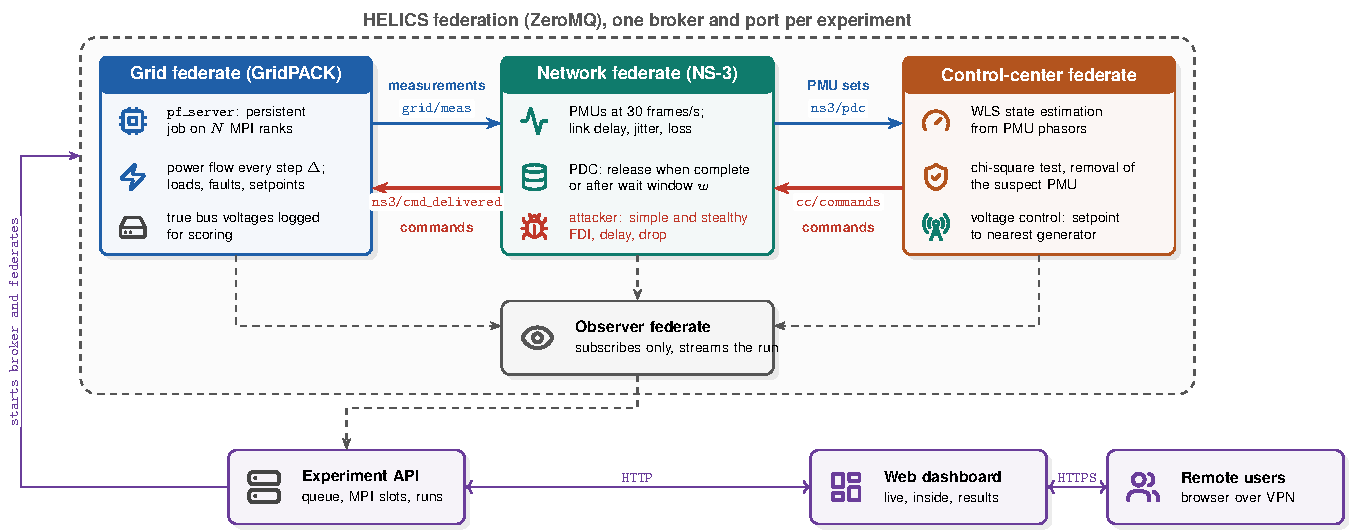
\includegraphics[width=0.86\textwidth]{fig_architecture.pdf}
\caption{Architecture of the testbed for one experiment. Solid blue arrows carry measurements, solid red arrows carry commands, and dashed arrows monitor and control the experiment.}
\label{fig:arch}
\end{figure*}

\begin{table}[t]
\caption{HELICS Publications}
\label{tab:topics}
\centering
\footnotesize
\begin{tabular}{@{}lP{2.1cm}P{3.5cm}@{}}
\toprule
Topic & From, to & Content \\
\midrule
grid/meas & grid, NS-3 & True phasors of every PMU channel, each grid step \\
ns3/pdc & NS-3, control center & Time-aligned PMU sets released by the PDC \\
cc/commands & control center, NS-3 & Generator setpoint commands \\
ns3/cmd\_delivered & NS-3, grid & Commands that reached the generator node, with arrival time \\
grid/status & grid, observer & True bus voltages, commands applied, solver report \\
ns3/status & NS-3, observer & Per-PMU frame counters, PDC and command counters \\
cc/status & control center, observer & Test result, removed PMUs, estimate, computing time \\
\bottomrule
\end{tabular}
\end{table}

\subsection{Grid Federate and the GridPACK Server}

GridPACK distributes a network over MPI processes, partitions it with ParMETIS and solves the network equations with PETSc \cite{palmer2016gridpack,karypis1998}. Its applications normally run once per study. A co-simulation needs a new solution at every grid step, and restarting an MPI job each step would spend most of the time on start-up and partitioning. We therefore wrote a small server, \texttt{pf\_server}, around GridPACK's power flow. It is started once per experiment with \texttt{mpirun}, reads the case and partitions the network once, and then waits for commands on the standard input of rank~0 (Table~\ref{tab:proto}). Rank~0 broadcasts each batch, each rank applies the changes to the buses it owns, GridPACK solves the power flow by Newton--Raphson with the MUMPS direct solver \cite{amestoy2001}, and the bus voltages are gathered to rank~0 \cite{mpi40}. Replies start with \texttt{@@} so that the driver can separate them from the solver's own output, which it passes to the dashboard. Zheng \emph{et al.} kept GridPACK's parallelism under HELICS in a similar way by making rank~0 the federate \cite{zheng2024hpc}. Our server keeps HELICS out of the MPI program, so the same driver can fall back to a built-in solver if the MPI job fails.

\begin{table}[t]
\caption{Protocol of \texttt{pf\_server}, One Exchange per Grid Step}
\label{tab:proto}
\centering
\footnotesize
\begin{tabular}{@{}P{1.2cm}P{3.5cm}P{2.9cm}@{}}
\toprule
Direction & Line & Meaning \\
\midrule
to rank 0 & \texttt{LOAD} bus P Q & new load at a bus \\
to rank 0 & \texttt{VSET} bus id V & new generator setpoint \\
to rank 0 & \texttt{SOLVE} / \texttt{QUIT} & solve the batch / stop \\
from rank 0 & \texttt{@@RANK} rank host buses branches & partition of each rank \\
from rank 0 & \texttt{@@READY} nbus nranks t\_setup & network read, partitioned \\
from rank 0 & \texttt{@@RESULT} ok nbus t\_apply t\_solve & solve finished, timings \\
from rank 0 & \texttt{@@V} bus Vm Va \dots{} \texttt{@@END} & voltage of every bus \\
\bottomrule
\end{tabular}
\end{table}

The grid federate is a Python program that drives the server. At every grid step $\Delta$ it applies the commands that have arrived over the network, updates the loads, solves, publishes the phasors, and logs the true voltage of every bus so that the experiment can be scored afterwards. Each load follows a slow sinusoid plus an independent random walk, which keeps the measurements from being constant. Events, such as the AVR fault used in this paper, are applied at their scheduled grid step.

\subsection{Network Federate: PMUs, Links and PDC}

Every PMU is an NS-3 node with its own point-to-point link to the control-center node. The one-way delay of link $i$ is drawn once per experiment as
\begin{equation}
d_i = L\,u_i, \qquad u_i \sim \mathcal{U}(0.5,\,1.5),
\label{eq:delay}
\end{equation}
where $L$ is the mean latency. Each frame also waits 2\,ms of processing plus a jitter drawn from $\mathcal{U}(0,2)$\,ms, and a packet error model loses frames with a fixed probability. Each generator has its own node and link, which carry commands.

At every frame time $kT$, each PMU takes the latest phasors published by the grid federate and adds noise. With $s$ the true phasor and $\epsilon_1, \epsilon_2 \sim \mathcal{N}(0,1)$, the reported phasor is
\begin{equation}
p = |s|\,(1 + 0.001\,\epsilon_1)\, e^{\,j(\angle s + 0.001\,\epsilon_2)}.
\label{eq:noise}
\end{equation}
The PMU sends the frame as a user datagram protocol (UDP) packet carrying its number, time stamp and phasors in JavaScript Object Notation (JSON). The PDC keeps a buffer per time stamp and releases a set as soon as every PMU has reported, or a wait window $w$ after the first frame of that time stamp arrived \cite{c37244}. A frame that arrives after its set was released is counted as late. Algorithm~\ref{alg:ns3} gives one frame interval, including the attacks of Section~\ref{sec:attacks}.

\begin{algorithm}[t]
\caption{Network federate, frame interval $k$}
\label{alg:ns3}
\begin{algorithmic}[1]
\Require frame period $T$, link delays $d_i$, wait window $w$, attack settings
\State request HELICS time $kT$
\State publish the PDC sets and command deliveries of the last interval
\State read new grid phasors $s_i$ and commands; send each command to its generator node
\State $a \gets$ attack active at $kT$
\If{$a$ is an FDI and the attacker holds the PMU at target bus $b$}
  \State $c \gets (v_f - |s_{b,0}|)\,e^{j \angle s_{b,0}}$ \Comment{adaptive offset}
\EndIf
\For{each PMU $i$}
  \State $p \gets s_i$ with noise by (\ref{eq:noise}); $e \gets 0$
  \If{$a$ and PMU $i$ is attacked}
    \If{drop} mark the frame dropped; \textbf{continue} \EndIf
    \If{FDI} add $h_{kb}\,c$ to attacked channels \EndIf
    \If{delay} $e \gets d_a$ \EndIf
  \EndIf
  \State send $p$ after $2\,\mathrm{ms} + \mathcal{U}(0,2)\,\mathrm{ms} + e$; the link adds $d_i$
\EndFor
\State run NS-3 events until $(k+1)T$; for each frame of time stamp $k'$ that reaches the PDC: if set $k'$ was released, mark it late; else store it, release set $k'$ if complete, and if it is the first frame of $k'$, schedule the release at arrival $+\,w$
\end{algorithmic}
\end{algorithm}

\subsection{PMU Placement}

A PMU at bus $i$ measures the voltage of $i$ and the current of every in-service branch at $i$, so it makes $i$ and its neighbours observable. With $A$ the bus connectivity matrix including the diagonal and $x \in \{0,1\}^n$ the placement, the testbed solves
\begin{equation}
\min_{x}\ \mathbf{1}^\top x \quad \text{s.t.} \quad A x \ge \kappa,
\label{eq:opp}
\end{equation}
as in \cite{gou2008}, where $\kappa_i = \min(k, \deg(i) + 1)$. Here $k = 1$ gives the minimum placement for full observability and $k = 2$ a redundant placement in which every bus is seen twice where its degree allows. The problem is solved with the HiGHS solver \cite{huangfu2018}. For the IEEE 118-bus system the minimum placement has 32 PMUs with 169 phasor channels (Fig.~\ref{fig:placemin}) and the redundant placement 68 PMUs with 315 channels (Fig.~\ref{fig:placered}). Bus 49, where the fault and the attacks of Section~\ref{sec:setup} take place, has a PMU in both. Under the minimum placement it is observed by PMUs 45 and 49, and under the redundant placement by PMUs 42, 45, 49, 51 and 66.

\begin{figure}[t]
\centering
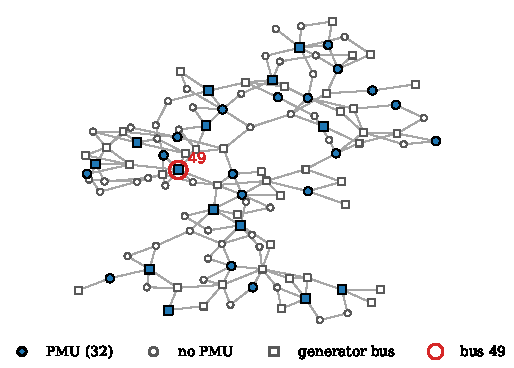
\includegraphics[width=\columnwidth]{fig_placement_min.pdf}
\caption{Minimum PMU placement for the IEEE 118-bus system computed by (\ref{eq:opp}) with $k = 1$: 32 PMUs.}
\label{fig:placemin}
\end{figure}

\begin{figure}[t]
\centering
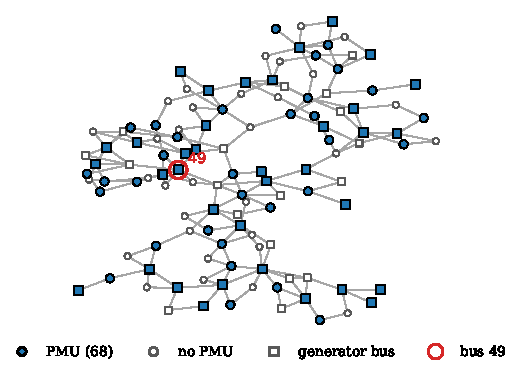
\includegraphics[width=\columnwidth]{fig_placement_red.pdf}
\caption{Redundant PMU placement for the IEEE 118-bus system computed by (\ref{eq:opp}) with $k = 2$: 68 PMUs.}
\label{fig:placered}
\end{figure}

\subsection{Control Center}

\emph{State estimation.} With all quantities complex, the channels of the received PMUs satisfy $z = HV + e$, where a row of $H$ is a unit vector for a voltage channel and a row of the branch admittance matrices for a current channel. The WLS estimate is
\begin{equation}
\hat V = G^{-1} H^{\mathsf H} W z, \qquad G = H^{\mathsf H} W H,
\label{eq:wls}
\end{equation}
with $W = \mathrm{diag}(1/\sigma_k^2)$ and $\sigma_k = \max(\sigma |z_k|, 10^{-4})$. $G$ is Hermitian positive definite and is factorized once per set with a sparse LU in symmetric mode. A set is observable when every bus is the own bus or a neighbour of a received PMU. When it is not, the estimator adds weak pseudo-measurements equal to the previous estimate with standard deviation 0.05\pu, so that it still returns a full state, and the set is not tested.

\emph{Bad data detection and removal.} For an observable set, the statistic
\begin{equation}
J = \sum_{k=1}^{m} \frac{|z_k - h_k \hat V|^2}{\sigma_k^2}
\label{eq:J}
\end{equation}
is compared with $\tau = \chi^2_{2m-2n}(1-\alpha)$ \cite{abur2004se}. For the IEEE 118-bus system with $\alpha = 0.01$, $\tau = 138.1$ with minimum placement and 462.2 with redundant placement. On an alarm, the control center computes the normalized residuals \cite{handschin1975}
\begin{equation}
r^N_k = \frac{|r_k|}{\sqrt{\Omega_{kk}}}, \qquad \Omega = R - H G^{-1} H^{\mathsf H},
\label{eq:lnr}
\end{equation}
with $R = W^{-1}$, removes all channels of the PMU that holds the largest one, estimates again and repeats the test, up to three PMUs. Removing every channel of that PMU matches the threat, since an attacker who controls a PMU controls all its channels.

\emph{Voltage control.} If the final estimate is free of alarms, the control center checks every bus against the limits $[v_{\min}, v_{\max}]$ with a dead band $\delta$. For a bus outside the limits it picks the in-service generator with the fewest branches to that bus and moves its setpoint by one step in the direction that corrects the violation, within the setpoint range and at most once per cooldown period per generator. While an alarm remains after removal, no command is sent, because the estimate cannot be trusted. Algorithm~\ref{alg:cc} gives the procedure for one set.

\begin{algorithm}[t]
\caption{Control center, one PDC set}
\label{alg:cc}
\begin{algorithmic}[1]
\Require set $S$ of received PMUs, $H$, $\sigma$, $\alpha$, limits $[v_{\min}, v_{\max}]$, dead band $\delta$, step $\Delta v$
\State $R \gets \emptyset$ \Comment{removed PMUs}
\State estimate $\hat V$ from $S$ by (\ref{eq:wls})
\State \textbf{if} $S$ is not observable \textbf{then} add pseudo-measurements; $\mathit{alarm} \gets$ false
\State \textbf{else} compute $J$ by (\ref{eq:J}) and $\tau$; $\mathit{alarm} \gets J > \tau$
\While{$\mathit{alarm}$ and $|R| < 3$ and removal is enabled}
  \State compute $r^N$ by (\ref{eq:lnr}); $p \gets$ PMU with the largest $r^N_k$
  \State $R \gets R \cup \{p\}$; drop all channels of $p$ from $S$
  \State re-estimate and re-test as in lines 2--4
\EndWhile
\If{$\mathit{alarm}$} \State \Return \Comment{hold control while bad data remain} \EndIf
\For{each bus $i$ with $|\hat V_i| > v_{\max} + \delta$ or $|\hat V_i| < v_{\min} - \delta$}
  \State $g \gets$ in-service generator nearest to $i$ in branches
  \If{no command was sent to $g$ within the cooldown}
    \State $v_g \gets$ $v_g \mp \Delta v$, clipped to the setpoint range
    \State publish $(g, v_g)$ on \texttt{cc/commands}
  \EndIf
\EndFor
\end{algorithmic}
\end{algorithm}

\subsection{Attack Models}
\label{sec:attacks}

The attacker targets a bus $b$ and wants the control center to see $|V_b| = v_f$. In the linear model this is the state change $\Delta V = c\,e_b$ with $c = (v_f - |V_b|)\,e^{j\theta_b}$, which changes channel $k$ by $h_{kb}\,c$. Four attacks act on the frames of the attacked PMUs between a start and an end time. The \emph{simple FDI} changes one channel, the voltage channel of the PMU at $b$ if there is one. The other channels still describe the true state, so the set becomes inconsistent. The \emph{stealthy FDI} adds $a = H\Delta V$, that is $h_{kb}\,c$ to every channel with $h_{kb} \ne 0$. Then the residual is unchanged and so is $J$ \cite{liu2009fdi}. It needs every PMU that has such a channel. In both cases, an attacker who holds the PMU at $b$ reads the true $V_b$ from each frame and recomputes $c$, so the injection follows the grid. The \emph{delay} attack holds the frames of every PMU with a channel that depends on $V_b$ for an extra $d_a$, and the \emph{drop} attack discards them. The attacker knows $H$ and the operating point, which is the full-knowledge case of \cite{liu2009fdi} and a bound on what the defenses can do.

\subsection{Time Coupling and Closed-Loop Latency}
\label{sec:time}

All federates use the HELICS ZeroMQ core. The grid federate requests the times $j\Delta$. The network federate requests the frame times $kT$ one after another, runs the NS-3 event queue up to the next frame time, and at each granted time first publishes what the previous interval produced and then reads new phasors and commands. The control center does not step on its own. HELICS wakes it whenever a new PDC set is published. The grid and network federates are uninterruptible, so they are granted only the times they request.

This scheme fixes the latency of the loop. Suppose an event changes the grid at $t_0 = j\Delta$. Both the grid and the network federate are granted $t_0$, and the network federate samples the phasors that were current before the grid published its new solution, so the event first appears in the frame stamped $t_0 + T$. If the PDC releases that set within one frame period, the network federate publishes it at $t_0 + 2T$, and the control center issues its command at that time. NS-3 reads the command at its next step and delivers it after the generator link delay $d_g$, and the grid applies it at its next step. The command therefore takes effect at
\begin{equation}
t_{\mathrm{apply}} = \Delta \left\lceil \frac{t_0 + 3T + d_g + \epsilon}{\Delta} \right\rceil,
\label{eq:loop}
\end{equation}
where $\epsilon$ is the processing and jitter delay. With $T = 33.3$\,ms, $\Delta = 0.5$\,s and $d_g$ of a few tens of milliseconds, any violation the control center can see is corrected one grid step after it appears. Fig.~\ref{fig:timeline} shows the timeline logged in the base experiment. The one-frame lag between grid and PMUs is a property of the time coupling. It could be removed by letting the network federate request a time just after the grid's, at the cost of a second synchronization per frame. We kept the simpler scheme and report the lag.

\begin{figure}[t]
\centering
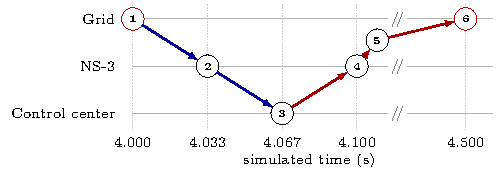
\includegraphics[width=\columnwidth]{fig_timeline.pdf}
\caption{Closed-loop timeline of the base experiment with the AVR fault at 4\,s, as logged ($L = 10$\,ms, $w = 20$\,ms). (1) The grid applies the fault. (2) First PMU frame that carries it. (3) The control center receives the set and issues the command. (4) NS-3 reads the command. (5) The command reaches the generator node at 4.107\,s. (6) The grid applies it at its next step.}
\label{fig:timeline}
\end{figure}

\subsection{Operating Layer and Dashboard}
\label{sec:ops}

An experiment is described by a scenario: grid, duration, MPI ranks, PMU placement and rate, network parameters, event, attack and control settings. Scenarios are entered in a form on the dashboard or uploaded as YAML files of up to 50 experiments that share common fields. The service checks each scenario against the chosen grid and rejects it with the name of the wrong field.

The service runs a set number of experiments at the same time, but starts an experiment only when its GridPACK ranks fit in the free MPI slots of the compute nodes. MPI ranks busy-wait for messages, so oversubscribed cores would slow every run that shares them. For each experiment the service creates a run directory on the shared file system, picks a free HELICS port, writes the configuration of each federate and starts the broker and the federates over the secure shell (SSH) on the nodes set on the Cluster page (Fig.~\ref{fig:cluster}). GridPACK's ranks are spread over the nodes through an MPI host file. If a federate fails, the others are stopped and the end of its log is shown in the queue.

The observer writes the state of the run about twice per second. The Live page shows the true and estimated voltages, the chi-square test, PDC completeness and each command. The Inside page shows what each engine computes, such as the partition of the MPI ranks, the Newton--Raphson mismatch, frames per PMU and the test before and after removal (Fig.~\ref{fig:inside}). The Results page opens finished runs. Every run is a directory of plain files (frames, sets, estimates, commands, true voltages and summaries), so results can be analysed outside the dashboard. All figures and tables of Section~\ref{sec:results} were produced from these files by scripts that are published with the paper. The dashboard and the application programming interface (API) are protected by authentication, and remote users reach the head node through the institution's virtual private network (VPN) or an SSH tunnel.

\begin{figure}[t]
\centering
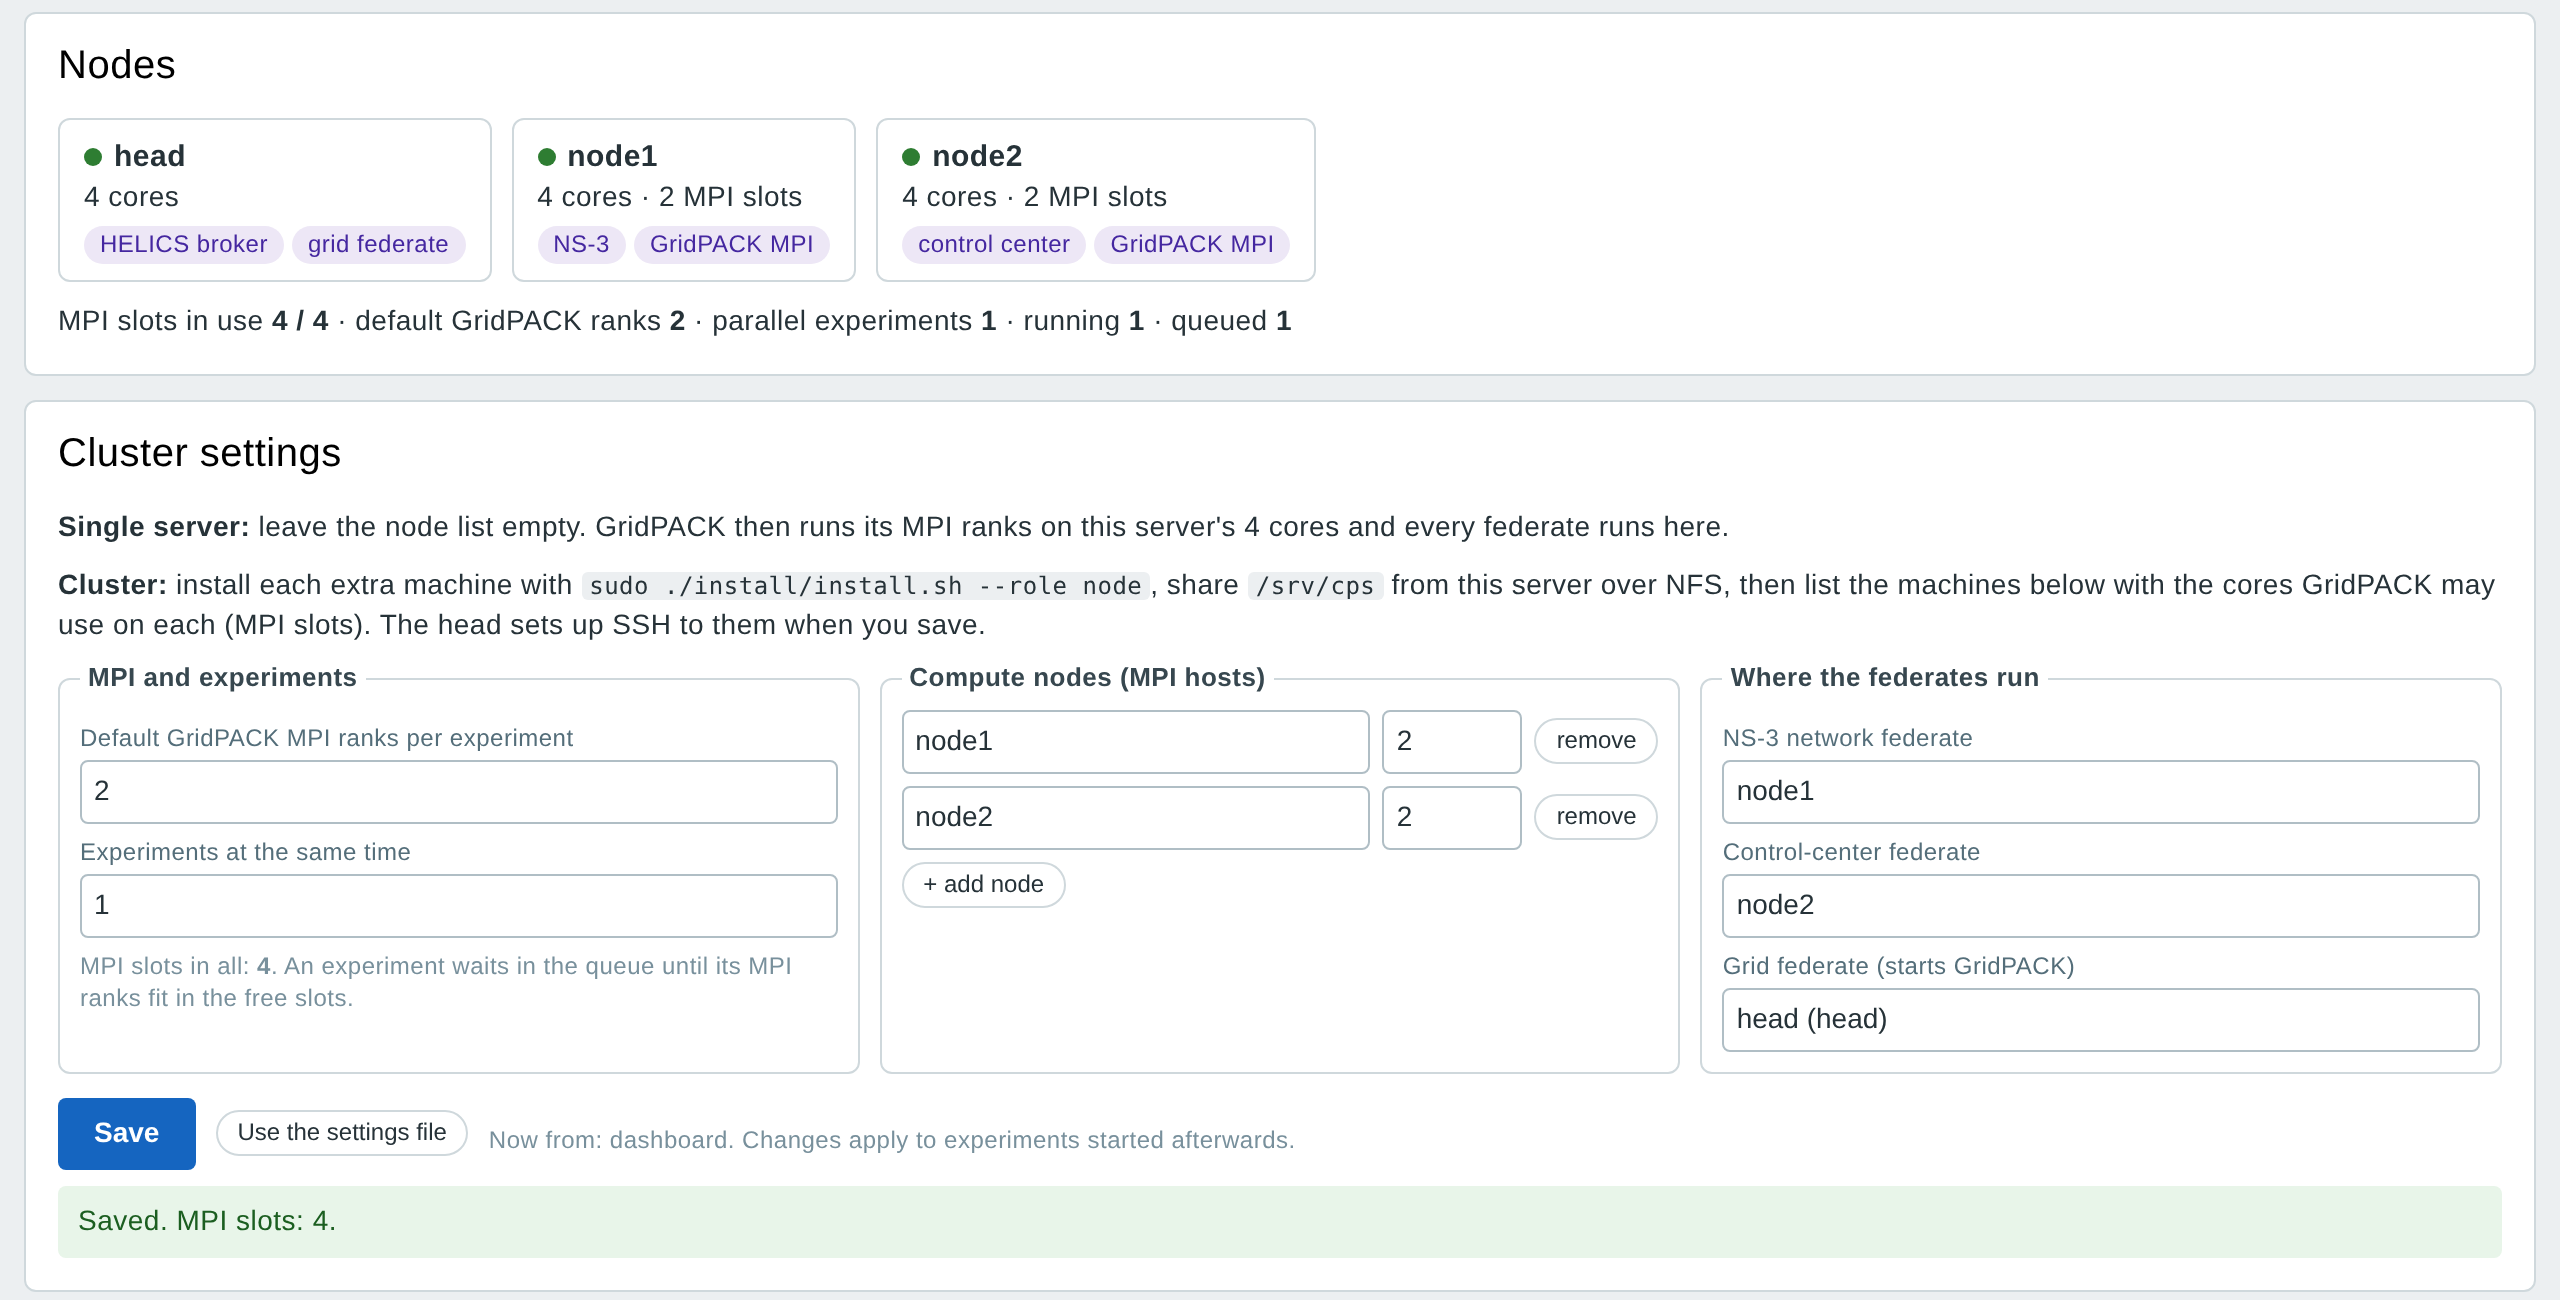
\includegraphics[width=\columnwidth]{fig_dashboard_cluster.png}
\caption{Cluster page of the dashboard: nodes with their roles, MPI slots in use, the queue, and the settings for default ranks, experiments at the same time and the node of each federate.}
\label{fig:cluster}
\end{figure}

\begin{figure}[t]
\centering
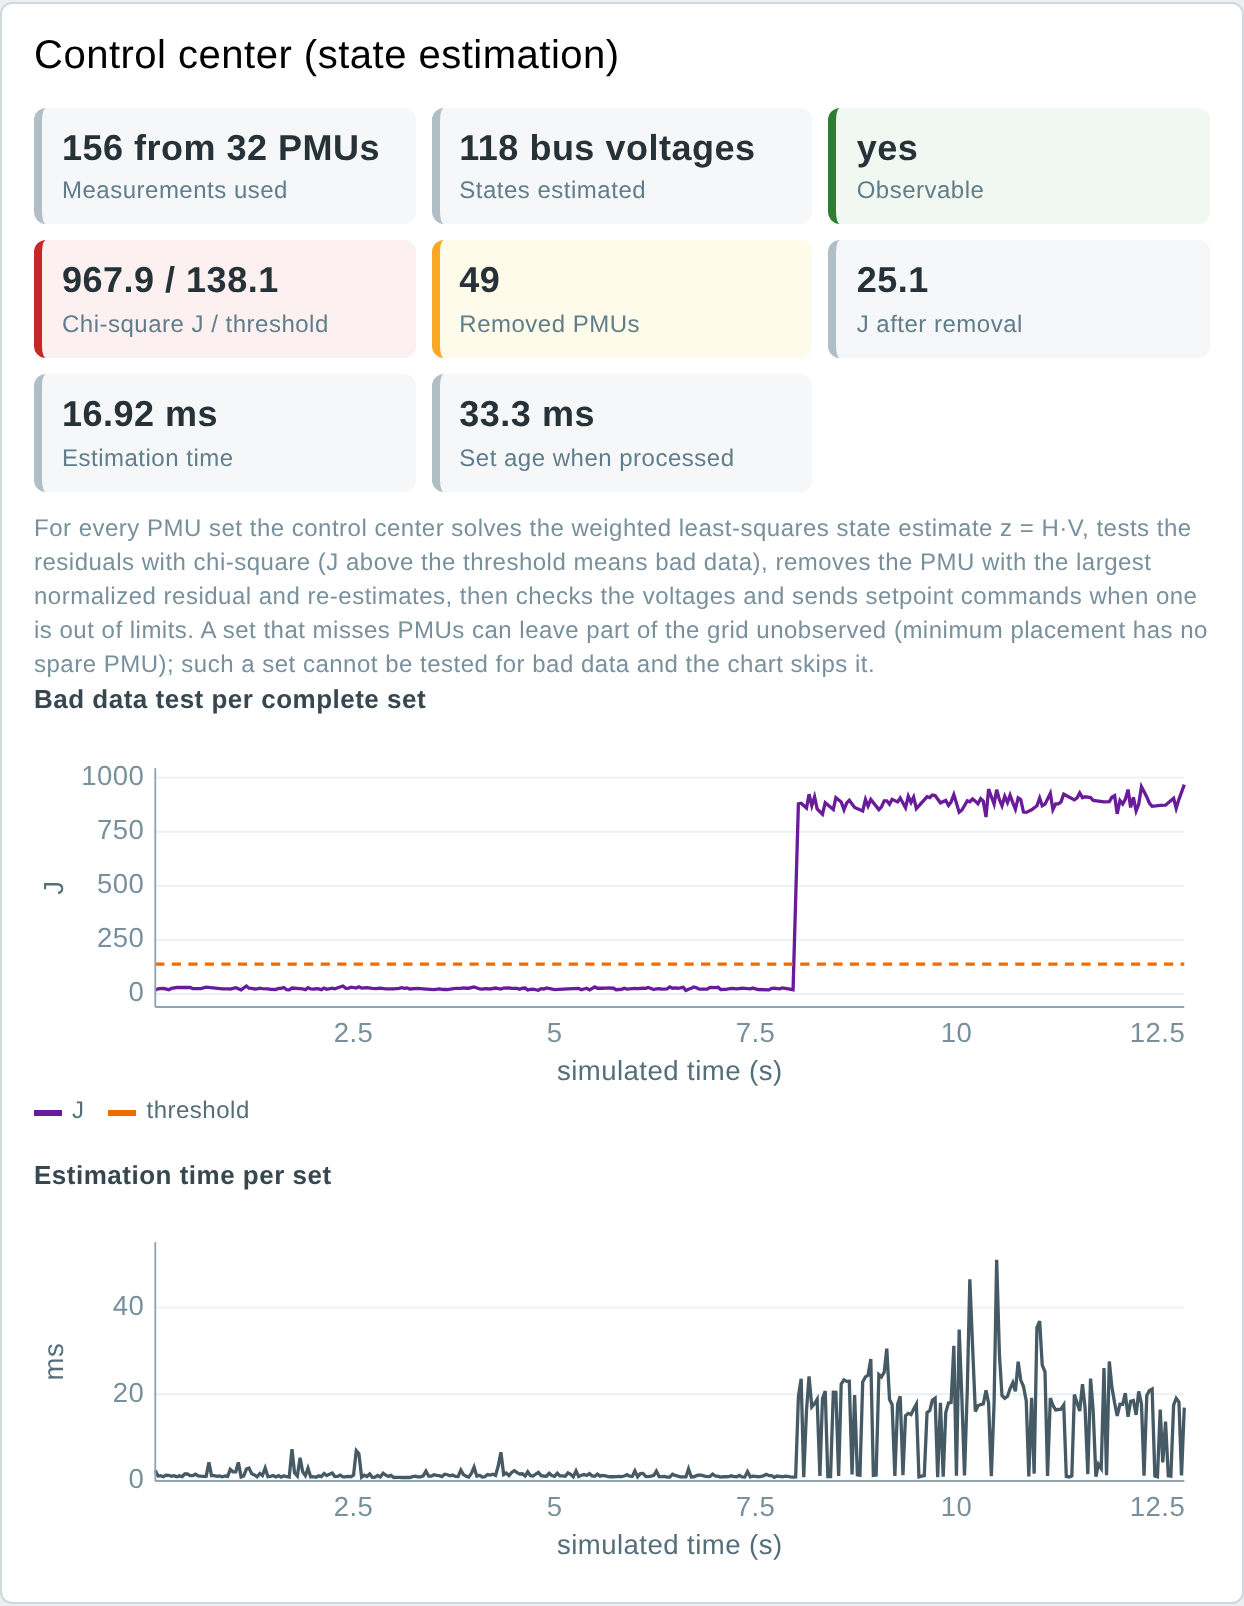
\includegraphics[width=0.82\columnwidth]{fig_dashboard_inside_cc.png}
\caption{Control-center panel of the Inside page during a simple FDI on bus 49 in a 30\,s IEEE 118-bus run: measurements used, chi-square test before and after removing PMU 49, and estimation time per set.}
\label{fig:inside}
\end{figure}

\section{Implementation and Experimental Setup}
\label{sec:setup}

\subsection{Test System and Preprocessing}

All experiments use the IEEE 118-bus system, taken from the MATPOWER case file \cite{zimmerman2011}. It has 118 buses, 186 branches and 54 generators. The testbed converts the case to GridPACK's input format and to a topology file used by the placement, the estimator and the network federate, and checks that both solvers agree on the base case before a grid is accepted. No other data set is involved. Every measurement in the study is generated by the co-simulation.

\subsection{Hardware and Software}

The testbed ran as a virtual cluster of three containers, a head node and two compute nodes with two MPI slots each, on one machine with four cores of an Intel Xeon processor at 2.1\,GHz and 15\,GB of memory. Fig.~\ref{fig:deploy} shows the placement of each part, and Table~\ref{tab:sw} lists the software. Two experiments ran at a time. The same build scripts install the testbed natively on Ubuntu or as a container image.

\begin{figure}[t]
\centering
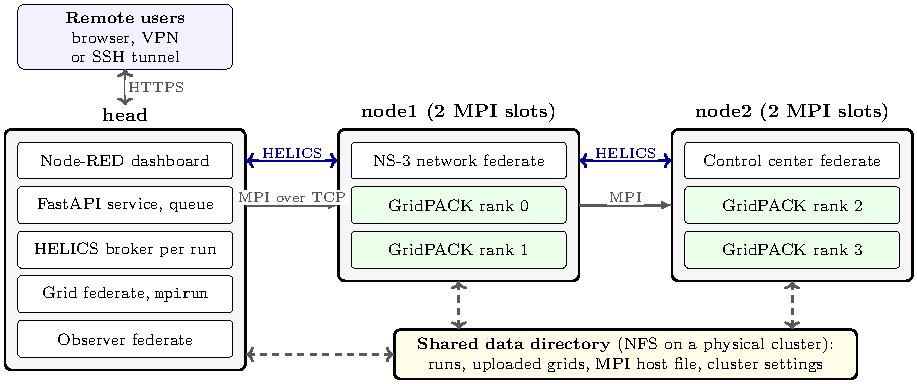
\includegraphics[width=\columnwidth]{fig_deployment.pdf}
\caption{Deployment on the three-node cluster used in this paper. GridPACK's ranks can span both compute nodes.}
\label{fig:deploy}
\end{figure}

\begin{table}[t]
\caption{Software Used in the Testbed}
\label{tab:sw}
\centering
\footnotesize
\begin{tabular}{@{}lP{4.8cm}@{}}
\toprule
Component & Software \\
\midrule
Grid simulation & GridPACK 3.5, PETSc 3.19, MUMPS, ParMETIS \\
Parallel runtime & Open MPI 4.1.6 \\
Network simulation & NS-3.48 \\
Co-simulation & HELICS 3.6.1, ZeroMQ core \\
Control center, API & Python 3.12, NumPy, SciPy, FastAPI \\
Dashboard & Node-RED 4.1, Dashboard 2.0 \\
Operating system & Ubuntu 24.04 \\
\bottomrule
\end{tabular}
\end{table}

\subsection{Scenarios and Parameters}

The base scenario lasts 10\,s with $\Delta = 0.5$\,s, 30 frames per second, $L = 10$\,ms, $w = 20$\,ms, no random loss, and GridPACK on one MPI rank. At 4\,s the AVR of generator 49 fails and moves its setpoint from 1.025 to 1.12\pu, which raises bus 49 above the upper limit of 1.08\pu. Every attack targets bus 49 from 4 to 9\,s. Both injections try to make the control center see $|V_{49}| = 1.02$\pu, a normal value. Table~\ref{tab:params} lists the parameters. From this base, 21 scenarios vary one factor at a time: the attack (none, simple FDI, stealthy FDI, delay of 100\,ms, drop), the placement (32 or 68 PMUs), random frame loss (0 or 5\%), the mean latency $L$ (5, 10, 20, 40, 80\,ms) and, at $L = 40$\,ms, the wait window $w$ (10, 20, 40, 60, 80\,ms). Each scenario ran with seeds 1 to 10. The seed sets the link delays (\ref{eq:delay}), the jitter, the loss, the measurement noise (\ref{eq:noise}) and the random walk of the loads. Another 15 runs repeated the base scenario with 1, 2 and 4 MPI ranks and seeds 1 to 5. All 225 runs were defined in one scenario file and submitted through the API.

\begin{table}[t]
\caption{Parameters of the Base Scenario}
\label{tab:params}
\centering
\footnotesize
\begin{tabular}{@{}P{4.1cm}P{3.6cm}@{}}
\toprule
Parameter & Value \\
\midrule
Duration, grid step $\Delta$ & 10\,s, 0.5\,s \\
PMU rate & 30 frames/s \\
Mean link latency $L$, spread & 10\,ms, $\pm50\%$ \\
Processing delay, jitter & 2\,ms, $\mathcal{U}(0,2)$\,ms \\
PDC wait window $w$ & 20\,ms \\
Noise & 0.1\% magnitude, 0.001\,rad \\
Estimator $\sigma$, test level $\alpha$ & 0.002, 0.01 \\
Pseudo-measurement deviation & 0.05\pu \\
Limits $[v_{\min}, v_{\max}]$, dead band $\delta$ & 0.94--1.08\pu, 0.003\pu \\
Setpoint step, range, cooldown & 0.01\pu, 0.95--1.10\pu, 1\,s \\
Load variation & 2\% sinusoid, 20\,s period, random walk \\
Event & AVR fault, generator 49, 1.12\pu{} at 4\,s \\
Attack window, target, $v_f$ & 4--9\,s, bus 49, 1.02\pu \\
Delay attack $d_a$ & 100\,ms \\
GridPACK MPI ranks & 1 (2 and 4 in Section~\ref{sec:compute}) \\
\bottomrule
\end{tabular}
\end{table}

\subsection{Baselines and Ablations}

Two baselines bound the results. \emph{No control} runs the same fault with the estimator and test but without voltage control, and gives the violation that the loop must remove. \emph{Control without attack} gives the best the loop can do. The proposed configuration, with the chi-square test, removal of up to three PMUs and voltage control, is then compared with three ablations. \emph{Detection without removal} keeps the test but holds control on every alarm, as a control center without identification would. \emph{Minimum versus redundant placement} removes the extra PMUs. \emph{PDC wait window} and \emph{link latency} sweeps change the timing of the PDC and the network. For the computing layer, the MPI sweep compares one, two and four ranks.

\subsection{Metrics and Statistical Procedure}

For each run we record the \emph{violation time}, the time during which the true voltage of some bus was outside the limits. It is measured at the grid steps and so has a resolution of 0.5\,s. We also record the time the first command was issued, the share of PDC sets that were complete and the share that were observable, and the number of sets whose first test raised an alarm and the number still in alarm after removal. On the network side we record the share of frames that arrived in time, their latency, and the mean delay of the PDC release after the time stamp. Finally we record the mean absolute error of the estimate and the GridPACK solve time per step. For each scenario we report the mean and standard deviation over the ten seeds and a 95\% confidence interval from Student's $t$ distribution. Differences between a scenario and its reference are tested with a two-sided exact permutation test on the difference of means, which needs no assumption about the distribution and remains valid when many runs give the same value. We also give the difference of means with a 95\% confidence interval. When all runs of both groups give the same value, the test cannot reject equality, and we say so.

\section{Results}
\label{sec:results}

\subsection{Validation of the Grid Solution}

The base scenario was run once more with the testbed's built-in Newton--Raphson solver in place of GridPACK. At all 21 grid steps, the true voltages of the 118 buses were identical to the six decimals logged, both for GridPACK on one rank and for GridPACK on four ranks split over the two compute nodes. The partition, the MPI exchange and the restart-free server therefore do not change the solution.

\subsection{Closed Loop Without Attack}

Fig.~\ref{fig:v49ctl} shows bus 49 in the two baselines. Without control the fault keeps $|V_{49}|$ near 1.12\pu{} to the end of the run, a violation of 6.5\,s. With control, the command for generator 49 was issued at 4.067\,s, delivered at 4.107\,s and applied at 4.5\,s, as predicted by (\ref{eq:loop}) and shown in Fig.~\ref{fig:timeline}. It lowered the setpoint to 1.015\pu, and the violation lasted one grid step, 0.5\,s. The same times were logged in all ten seeds. All 9568 frames of each run arrived in time, with a median latency of 12.8\,ms and a 95th percentile of 17.3\,ms (means over seeds), and the PDC released each set 17.9\,ms after its time stamp on average. The mean absolute error of the estimate was $2.8\times10^{-4}$\pu, and no set raised an alarm.

\begin{figure}[t]
\centering
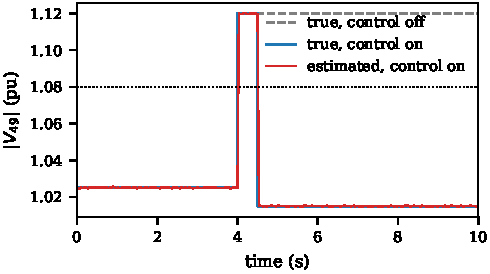
\includegraphics[width=\columnwidth]{fig_v49_control.pdf}
\caption{Voltage of bus 49 without and with voltage control, and the control center's estimate (seed 1). The dotted line is the 1.08\pu{} limit.}
\label{fig:v49ctl}
\end{figure}

\begin{table*}[t]
\caption{Attacks and PMU Placement, IEEE 118-Bus System, AVR Fault at Generator 49 at 4\,s, Attacks on Bus 49 From 4 to 9\,s. Mean $\pm$ Standard Deviation Over Ten Seeds; a Single Value Means All Seeds Gave the Same Result}
\label{tab:attacks}
\centering
\footnotesize
\begin{tabular}{@{}llcccccc@{}}
\toprule
Case & Attacked PMUs (bus) & Complete & Observable & Alarm sets & Alarm sets & First command & Violation \\
 & & sets (\%) & sets (\%) & (first test) & (after removal) & issued (s) & time (s) \\
\midrule
\multicolumn{8}{@{}l}{\emph{Minimum placement, 32 PMUs}} \\
No control (baseline) & -- & 100.0 & 100.0 & 0 & 0 & -- & 6.5 \\
Control, no attack (baseline) & -- & 100.0 & 100.0 & 0 & 0 & 4.067 & 0.5 \\
Simple FDI & 49 & 100.0 & 95.0 & 15 & 0 & 4.067 & 0.5 \\
Simple FDI, no removal & 49 & 100.0 & 100.0 & 149 & 149 & 9.033 & 5.5 \\
Stealthy FDI & 45, 49 & 100.0 & 100.0 & 0 & 0 & 4.067 & 0.5 \\
Delay 100\,ms & 45, 49 & 49.7 & 49.7 & 0 & 0 & 9.033 & 5.5 \\
Drop & 45, 49 & 49.7 & 49.7 & 0 & 0 & 9.033 & 5.5 \\
5\% frame loss & -- & 20.5\,$\pm$\,1.5 & 20.5\,$\pm$\,1.5 & 0 & 0 & 4.067 & 0.5 \\
\midrule
\multicolumn{8}{@{}l}{\emph{Redundant placement, 68 PMUs}} \\
Simple FDI & 49 & 100.0 & 100.0 & 15 & 0 & 4.067 & 0.5 \\
Stealthy FDI & 42, 45, 49, 51, 66 & 100.0 & 100.0 & 0 & 0 & 4.067 & 0.5 \\
Delay 100\,ms & 42, 45, 49, 51, 66 & 49.7 & 49.7 & 0 & 0 & 4.067 & 0.5 \\
Drop & 42, 45, 49, 51, 66 & 49.7 & 49.7 & 0 & 0 & 4.067 & 0.5 \\
5\% frame loss & -- & 3.0\,$\pm$\,0.8 & 85.3\,$\pm$\,2.0 & 0 & 0 & 4.067 & 0.5 \\
\bottomrule
\end{tabular}
\end{table*}


\subsection{Attacks and PMU Placement}

Table~\ref{tab:attacks} lists the 13 scenarios on attacks and placement, and Fig.~\ref{fig:violation} shows the violation time with its 95\% confidence interval. In these scenarios the random factors changed the frames, delays and noise but never the outcome, so every seed gave the same violation time and the same command time.

\begin{figure}[t]
\centering
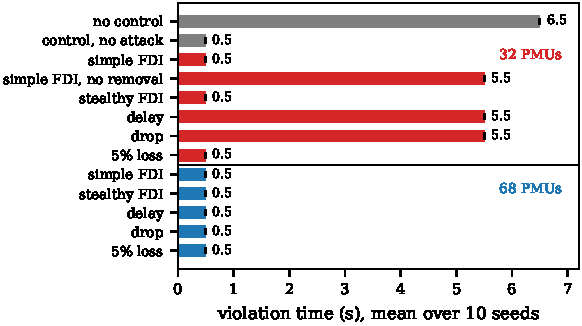
\includegraphics[width=\columnwidth]{fig_violation.pdf}
\caption{Violation time per scenario, mean over ten seeds with 95\% confidence interval. Red: 32 PMUs; blue: 68 PMUs; grey: baselines.}
\label{fig:violation}
\end{figure}

\emph{Simple FDI with 32 PMUs.} The attacker holds PMU 49 and replaces its voltage channel. In the set stamped 4.000\,s the fault is not yet visible and the falsified 1.02\pu{} is close to the true 1.025\pu, so $J = 36$ (seed 1). In the next set the true voltage is 1.12\pu, the channel still reads 1.02\pu, and the current channels disagree with it. $J$ rose to 2414 against a threshold of 138.1 (Fig.~\ref{fig:chi2}). The largest normalized residual pointed to PMU 49, which was removed, and the new estimate put bus 49 at 1.119\pu{} (Fig.~\ref{fig:profile}). The command was issued at 4.067\,s, as without attack. After the command took effect, the true voltage was 1.015\pu, close to the value the attacker reported, so $J$ fell below the threshold for the rest of the attack. This is why exactly 15 sets, $0.5\,\mathrm{s} \times 30$\,sets/s, raised an alarm in every seed. Removing PMU 49 left some buses without an observing PMU in those 15 sets, so the final estimate could not be tested again. The control center acted on an estimate completed with pseudo-measurements, which explains the 95.0\% of observable sets. The command was correct, but the test that would have confirmed it was not run.

\emph{Detection without removal.} With the same attack and the test in place but no removal, every set from 4.033 to 9.0\,s raised an alarm. The estimate of bus 49 stayed near the truth, at 1.116\pu{} on average in seed 1, because the current channels outweighed the single false voltage channel. The control center nevertheless held its commands while the alarm stood. The command came only after the attack ended, at 9.033\,s, and the violation lasted 5.5\,s in every seed. Detection without identification protected the estimate and blocked the control.

\emph{Stealthy FDI.} Bus 49 is observed by PMU 49 and by the current that PMU 45 measures on branch 45--49, so the stealthy attack changed both. As expected, $J$ did not move and stayed below 36 during the attack (Fig.~\ref{fig:chi2}), and the estimate of bus 49 stayed at 1.02\pu{} (Fig.~\ref{fig:v49att}). The attack still failed to hide the fault. Shifting the estimate of bus 49 cannot also hide the fault's effect on the neighbouring buses, whose measurements are untouched. The control center estimated bus 48 at 1.096\pu, issued the command because of that bus at 4.067\,s, and the command went to generator 49, the generator nearest to bus 48.

\emph{Delay and drop.} Delaying the frames of PMUs 45 and 49 by 100\,ms, five times the wait window, made them late for every set. Their sets were released without them, so 50.3\% of the sets were incomplete and unobservable. Bus 49 was then estimated from pseudo-measurements of the last value seen before the attack, 1.025\pu{} (Fig.~\ref{fig:v49att}), and the violation went unseen until the frames returned at 9\,s, giving 5.5\,s of violation in every seed. Dropping the frames had the same effect. For the control center, a frame that arrives after the window is a lost frame.

\emph{Redundant placement.} With 68 PMUs the simple FDI was detected in the same set and PMU 49 was removed. This time the grid stayed observable after removal and the second test passed ($J = 77$ against 434 in seed 1). The stealthy FDI now needed five PMUs and was again not detected, but the neighbours exposed the fault. Under delay and drop of all five PMUs that observe bus 49, bus 48 remained observed through other PMUs and was estimated at 1.096\pu, and the command was issued at 4.067\,s. Every attack in the set left the violation at 0.5\,s.

\emph{Random loss.} With 5\% of frames lost on every link, only 20.5\% of the 32-PMU sets were complete. Because the loss was spread over all PMUs, the frames of bus 49's PMUs arrived in most sets, and the violation was corrected as without loss. With 68 PMUs only 3.0\% of the sets were complete, since a set needs all 68 frames, but 85.3\% were still observable, against 20.5\% with 32 PMUs.

\begin{figure}[t]
\centering
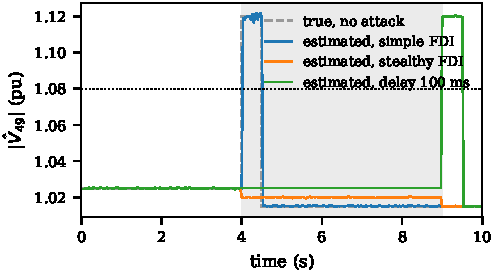
\includegraphics[width=\columnwidth]{fig_v49_attacks.pdf}
\caption{Estimate of bus 49 under three attacks with 32 PMUs (seed 1). Under the simple FDI the estimate follows the true voltage. Shaded: attack window.}
\label{fig:v49att}
\end{figure}

\begin{figure}[t]
\centering
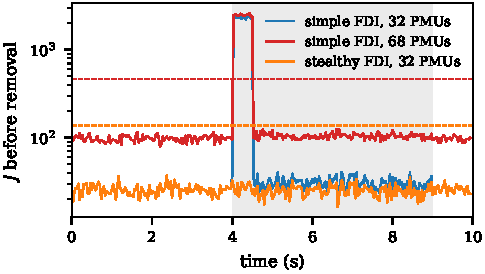
\includegraphics[width=\columnwidth]{fig_chi2.pdf}
\caption{Chi-square statistic before removal (solid) and threshold (dashed) for each case, seed 1. The simple FDI is detected from 4.033 to 4.5\,s with both placements. The stealthy FDI leaves $J$ unchanged. Shaded: attack window.}
\label{fig:chi2}
\end{figure}

\begin{figure}[t]
\centering
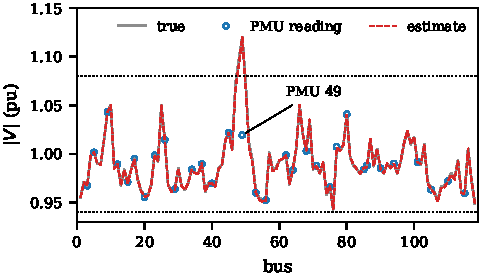
\includegraphics[width=\columnwidth]{fig_profile.pdf}
\caption{Voltage of every bus in the set stamped 4.1\,s, simple FDI on bus 49, 32 PMUs, seed 1: true voltage of the state the PMUs sampled, PMU readings, and the estimate after PMU 49 was removed. PMU 49 reported 1.019\pu{} for a true 1.120\pu.}
\label{fig:profile}
\end{figure}

\subsection{Network Latency and the PDC Wait Window}

\begin{table*}[t]
\caption{Effect of Mean Link Latency $L$ and PDC Wait Window $w$, IEEE 118-Bus System, Minimum Placement, AVR Fault, No Attack. Mean $\pm$ Standard Deviation Over Ten Seeds}
\label{tab:latency}
\centering
\footnotesize
\begin{tabular}{@{}rrcccccccc@{}}
\toprule
$L$ & $w$ & Frames & Complete & Observable & Latency & Latency & PDC release & Estimation & Violation \\
(ms) & (ms) & in time (\%) & sets (\%) & sets (\%) & p50 (ms) & p95 (ms) & delay (ms) & error ($10^{-3}$\,pu) & time (s) \\
\midrule
5 & 20 & 100.0 & 100.0 & 100.0 & 7.8\,$\pm$\,0.4 & 10.2\,$\pm$\,0.3 & 10.5\,$\pm$\,0.1 & 0.28\,$\pm$\,0.00 & 0.5 \\
10 & 20 & 100.0 & 100.0 & 100.0 & 12.8\,$\pm$\,1.0 & 17.3\,$\pm$\,0.3 & 17.9\,$\pm$\,0.2 & 0.28\,$\pm$\,0.00 & 0.5 \\
20 & 20 & 98.6\,$\pm$\,1.3 & 67.8\,$\pm$\,26.9 & 67.8\,$\pm$\,26.9 & 22.8\,$\pm$\,1.8 & 31.5\,$\pm$\,0.7 & 32.5\,$\pm$\,0.2 & 0.29\,$\pm$\,0.02 & 0.5 \\
40 & 20 & 53.1\,$\pm$\,9.1 & 0.0 & 0.0 & 34.2\,$\pm$\,2.2 & 42.7\,$\pm$\,1.7 & 44.0\,$\pm$\,1.8 & 9.07\,$\pm$\,2.67 & 4.1\,$\pm$\,3.1 \\
80 & 20 & 25.7\,$\pm$\,8.2 & 0.0 & 0.0 & 53.9\,$\pm$\,4.6 & 62.1\,$\pm$\,5.0 & 65.4\,$\pm$\,3.5 & 16.33\,$\pm$\,2.00 & 5.9\,$\pm$\,1.9 \\
\midrule
40 & 10 & 25.8\,$\pm$\,8.2 & 0.0 & 0.0 & 28.3\,$\pm$\,2.3 & 32.5\,$\pm$\,2.5 & 34.0\,$\pm$\,1.8 & 15.99\,$\pm$\,2.09 & 5.9\,$\pm$\,1.9 \\
40 & 40 & 99.1\,$\pm$\,0.9 & 85.5\,$\pm$\,19.3 & 85.5\,$\pm$\,19.3 & 43.2\,$\pm$\,3.7 & 60.7\,$\pm$\,1.1 & 62.2\,$\pm$\,0.4 & 0.29\,$\pm$\,0.01 & 0.5 \\
40 & 60 & 99.7 & 100.0 & 100.0 & 43.3\,$\pm$\,3.7 & 60.9\,$\pm$\,1.1 & 62.2\,$\pm$\,0.4 & 0.28\,$\pm$\,0.00 & 0.5 \\
40 & 80 & 99.7 & 100.0 & 100.0 & 43.3\,$\pm$\,3.7 & 60.9\,$\pm$\,1.1 & 62.2\,$\pm$\,0.4 & 0.28\,$\pm$\,0.00 & 0.5 \\
\bottomrule
\end{tabular}
\end{table*}


Table~\ref{tab:latency} and Fig.~\ref{fig:latency} repeat the controlled run without attack at other mean latencies. Because each link delay is drawn between $0.5L$ and $1.5L$ by (\ref{eq:delay}), the spread of delays grows with $L$, while the wait window is measured from the first frame of a time stamp. Once the spread exceeds $w$, the slow links miss their sets. At $L = 20$\,ms the share of complete sets fell to $67.8 \pm 26.9$\% and depended strongly on the seed, between 28\% and 100\%, while 98.6\% of the frames still arrived in time. At $L = 40$\,ms no set was complete or observable in any seed, and whether the fault was seen depended on the delays drawn for PMUs 45 and 49. In seed 1, PMU 49's link had 32\,ms against a fastest link of 21\,ms, its frames fit in the window, and the command was issued at 4.100\,s. In seed 3 its link had 49.5\,ms against 20.1\,ms, its frames were always late, and the violation lasted to the end of the run. Over ten seeds the fault went unseen in six, and the violation averaged 4.1\,s with no attack at all. At $L = 80$\,ms the fault went unseen in nine seeds out of ten. The mean absolute error of the estimate rose from $2.8\times10^{-4}$\pu{} to $9.1\times10^{-3}$\pu{} at 40\,ms and $1.6\times10^{-2}$\pu{} at 80\,ms, because the unobserved buses were held near earlier values.

Fig.~\ref{fig:pdcwait} shows the remedy at $L = 40$\,ms. A wait window of 10\,ms made matters worse, with the fault unseen in nine seeds. A window of 40\,ms, equal to the expected spread $L$, restored $85.5 \pm 19.3$\% complete sets and corrected the fault in every seed, and 60\,ms restored all sets. The price is latency. The PDC released sets 62\,ms after their time stamp with $w \ge 40$\,ms, against 18\,ms at $L = 10$\,ms. Beyond 60\,ms, a longer window brought nothing, because every frame had already arrived. The wait window therefore has to follow the spread of the link delays, and their mean is a poor guide.

\begin{figure}[t]
\centering
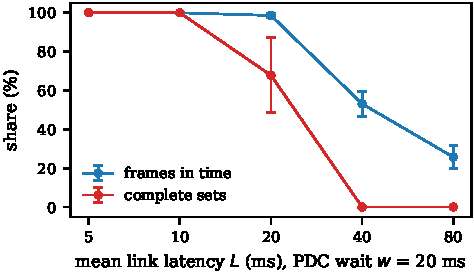
\includegraphics[width=\columnwidth]{fig_latency.pdf}
\caption{Share of frames that arrived in time and of complete PDC sets against the mean link latency, $w = 20$\,ms, mean over ten seeds with 95\% confidence interval.}
\label{fig:latency}
\end{figure}

\begin{figure}[t]
\centering
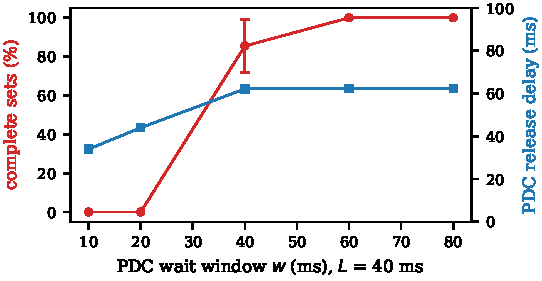
\includegraphics[width=\columnwidth]{fig_pdc_wait.pdf}
\caption{Complete sets (left axis) and mean PDC release delay after the time stamp (right axis) against the PDC wait window at $L = 40$\,ms, mean over ten seeds with 95\% confidence interval.}
\label{fig:pdcwait}
\end{figure}

\subsection{Ablation and Statistical Significance}

\begin{table}[t]
\caption{Statistical Tests Between Configurations, Ten Seeds Each. Difference of Means (B $-$ A) With 95\% Confidence Interval and Two-Sided Exact Permutation Test}
\label{tab:stats}
\centering
\footnotesize
\setlength{\tabcolsep}{3pt}
\begin{tabular}{@{}P{3.3cm}ccc@{}}
\toprule
Comparison (A vs.\ B) & Mean A & Mean B $-$ A & $p$ \\
\midrule
Voltage control (no control vs.\ control) & 0.5\,s & +6.0\,s & $1.1\times10^{-5}$ \\
Removal (simple FDI, 32 PMUs) & 0.5\,s & +5.0\,s & $1.1\times10^{-5}$ \\
Simple FDI with removal vs.\ no attack & 0.5\,s & +0.0\,s & 1 \\
Stealthy FDI vs.\ no attack (32 PMUs) & 0.5\,s & +0.0\,s & 1 \\
Placement under delay & 0.5\,s & +5.0\,s & $1.1\times10^{-5}$ \\
Placement under drop & 0.5\,s & +5.0\,s & $1.1\times10^{-5}$ \\
Placement under 5\% loss (observable sets) & 85.3\,\% & -64.8 [-66.4, -63.1]\,\% & $1.1\times10^{-5}$ \\
Latency 10 vs.\ 20\,ms (complete sets) & 100.0\,\% & -32.2 [-50.0, -14.3]\,\% & 0.003 \\
Wait 40 vs.\ 20\,ms at $L$ = 40\,ms (complete sets) & 85.5\,\% & -85.5 [-98.3, -72.7]\,\% & $1.1\times10^{-5}$ \\
Wait 40 vs.\ 10\,ms at $L$ = 40\,ms (violation) & 0.5\,s & +5.4 [+4.1, +6.7]\,s & $1.2\times10^{-4}$ \\
Latency 10 vs.\ 80\,ms (violation) & 0.5\,s & +5.4 [+4.1, +6.7]\,s & $1.2\times10^{-4}$ \\
\bottomrule
\end{tabular}
\end{table}


Table~\ref{tab:stats} tests the main comparisons. Removing the bad PMU, adding redundant PMUs against delay and drop, and closing the voltage loop each changed the violation time by 5.0 to 6.0\,s with $p = 1.1\times10^{-5}$, the smallest value an exact two-sided test can give with ten runs per group, since all twenty runs fell on the expected side. The simple FDI with removal and the stealthy FDI did not change the violation time compared with the attack-free run in any seed, so the test cannot reject equality ($p = 1$). For the network, the drop in complete sets from 10 to 20\,ms ($p = 0.003$), the gain from a 40\,ms instead of a 20\,ms window at $L = 40$\,ms, and the longer violations at 80\,ms latency or with a 10\,ms window ($p = 1.2\times10^{-4}$) were all significant at the 1\% level. Redundant placement under 5\% loss raised the observable sets by 64.8 percentage points (95\% confidence interval 63.1 to 66.4).

\subsection{Computing Time}
\label{sec:compute}

\begin{table}[t]
\caption{Computing Time per Experiment With 1, 2 and 4 GridPACK MPI Ranks, Base Scenario, Five Seeds Each (Mean $\pm$ Standard Deviation)}
\label{tab:mpi}
\centering
\footnotesize
\begin{tabular}{@{}lccc@{}}
\toprule
Ranks & Solve time (ms) & Grid step (ms) & Wall time (s) \\
\midrule
1 & 9.6\,$\pm$\,1.6 & 17.5\,$\pm$\,4.2 & 4.8\,$\pm$\,0.4 \\
2 & 32.6\,$\pm$\,10.5 & 52.1\,$\pm$\,18.7 & 6.1\,$\pm$\,0.6 \\
4 & 90.5\,$\pm$\,19.5 & 136.0\,$\pm$\,15.1 & 7.3\,$\pm$\,0.3 \\
\bottomrule
\end{tabular}
\end{table}

\begin{table}[t]
\caption{Control-Center Computing Time per PDC Set, IEEE 118-Bus System}
\label{tab:bench}
\centering
\footnotesize
\begin{tabular}{@{}llccc@{}}
\toprule
PMUs & Set & Median (ms) & p95 (ms) & Max (ms) \\
\midrule
32 & clean & 0.91 & 1.50 & 3.90 \\
32 & FDI, PMU 49 removed & 19.39 & 29.58 & 37.32 \\
68 & clean & 0.85 & 1.53 & 2.30 \\
68 & FDI, PMU 49 removed & 37.60 & 51.46 & 56.84 \\
\bottomrule
\end{tabular}
\end{table}


Table~\ref{tab:mpi} gives the GridPACK time per grid step and the wall-clock time of a 10\,s experiment with one, two and four ranks, while a second experiment ran at the same time. A 118-bus power flow takes about 10\,ms on one rank, so every additional rank adds more communication than it removes work, and four ranks split over two containers that exchange MPI messages over the transmission control protocol (TCP) needed 90\,ms per solve. For this grid one rank is the right choice, and the cluster pays off by running many experiments at once. The runs of the study took between 4.0 and 9.0\,s each, except the first two after the cluster started, which took 20\,s.

Table~\ref{tab:bench} gives the control center's time per set, measured by a benchmark of the estimator on the IEEE 118-bus system with 200 noisy sets per case. A clean set took a median of 0.9\,ms with either placement. When an alarm triggered the normalized-residual test, which needs one solve per channel, and a second estimate, the median rose to 19\,ms with 32 PMUs and 38\,ms with 68 PMUs, with a maximum of 57\,ms. These times do not affect the simulated time of a run, but they matter for a real-time version, because a frame period is 33.3\,ms.

\subsection{Comparison With Prior Work}

Direct numerical comparison with the platforms of Table~\ref{tab:compare} is limited, because they study other systems, events and metrics. Where the quantities match, the results agree. The median PMU-to-PDC latencies of 12.8\,ms at $L = 10$\,ms and 22.8\,ms at $L = 20$\,ms bracket the mean of about 20\,ms that Morato \emph{et al.} found for PMU traffic over 5G \cite{morato2024fiveg}. Our earlier IEEE 14-bus prototype reported latencies rising from 10 to about 100\,ms under denial of service but could not show the effect on the grid \cite{islam2024remotely}. The present study shows that a delay of that order hides an over-voltage for 5.5\,s under minimum placement. Zheng \emph{et al.} found that GridPACK under HELICS runs faster than real time for a 3000-bus system on four processes \cite{zheng2024hpc}. Our single-rank runs simulated 10\,s of a smaller system in about 5\,s of wall-clock time on shared cores, with the full network and control center in the loop. The value of the chi-square test against stealthy attacks matches \cite{liu2009fdi,yang2024tensor}: it did not react at all. The benefit of placement that keeps the grid observable without the attacked PMUs matches the analysis of \cite{khalafi2022intrusion}, here shown in a closed loop with a simulated network.

\emph{Calibration of the test.} The chi-square statistic in normal operation averaged 25.5 with minimum placement, between 24.7 and 26.3 over the seeds, well below its 102 degrees of freedom. The estimator assumes $\sigma = 0.002$ while the simulated noise is 0.001 in magnitude and 0.001\,rad in angle, so each real component of a residual has about a quarter of the variance that the test assumes, and $(2m - 2n)/4 \approx 26$. The test raised no false alarm in any of the 225 runs.

\section{Discussion}
\label{sec:disc}

\subsection{Interpretation}

The experiments separate the defenses by what they protect. The chi-square test with normalized-residual removal protects the estimate, and with it the control action, against a falsified channel, provided enough redundancy remains after removal to test the result again. Detection alone protects the estimate but blocks the control, which in this case cost five seconds of over-voltage in every seed. The stealthy injection did not raise the test at all, and it failed here only because it shifted one bus while the fault also raised the neighbouring buses. An attacker who falsifies the neighbourhood too would need more PMUs, and the learned detectors of \cite{chen2022datadriven,bhattacharjee2023deep} are one way to catch such attacks. Under minimum placement, delay and drop were the most effective attacks. Neither changes a value, and both turn a measurement into a missing one, which is consistent with the role of data dropout in time-synchronization attacks \cite{zadsar2023preventing,shereen2024topology}. Redundant placement neutralized them because it kept the neighbourhood of bus 49 observed, which is the condition Khalafi \emph{et al.} derived for locating attacks \cite{khalafi2022intrusion}. The PDC results agree with the observation that wait times must be set from the latency of the slowest stream \cite{pourramezan2021pdc}. A frame that arrives after the window is, for the control center, a lost frame.

\subsection{Limitations}

The cluster was virtual, three containers on four cores, so the MPI times include contention and TCP between containers and do not show what separate machines would give. The grid runs in quasi-steady state with a 0.5\,s step, which sets the resolution of the violation time and the delay before a command takes effect. The testbed also has a dynamic mode, which this paper does not use. The frames are JSON and do not follow IEEE C37.118.2, so real PMUs cannot yet join an experiment. The co-simulation runs as fast as it can and is not paced to wall-clock time. The PMU frames lag the grid by one frame, as explained in Section~\ref{sec:time}. The control center acts on an estimate once its alarm has cleared, even when the cleared estimate could not be tested because removal made the grid unobservable.

\subsection{Threats to Validity}

\emph{Internal validity.} The outcome depends on the time coupling. We derived the loop latency in (\ref{eq:loop}) and checked it against the logged times of every command. The grid solution was checked against an independent Newton--Raphson solver. Each scenario changed one factor from the base, and all runs used the same software build.

\emph{Construct validity.} The violation time is measured at grid steps, so differences smaller than 0.5\,s are not visible. The chi-square test assumes $\sigma = 0.002$ while the simulated noise is smaller (Section~\ref{sec:results}), which makes the test conservative. A smaller injection would be harder to detect than with matched weights.

\emph{Statistical validity.} Ten seeds per scenario vary noise, delays, loss and loads but not the fault or the attack, which are fixed by design. Many outcomes were therefore identical in all seeds. The tests show that the differences between these groups cannot be explained by the random factors, but they do not cover other faults, targets or attack sizes.

\emph{External validity.} All results come from one system, one fault and one target bus. Bus 49 is a well-connected generator bus. A bus with fewer neighbours, a different placement or a dynamic event could change the outcome, and the testbed can run those cases from the same scenario file.

\section{Conclusion and Future Work}
\label{sec:concl}

This paper presented an open-source testbed in which GridPACK on MPI, NS-3 with a PMU network and a PDC, and a control center with state estimation, bad data detection and voltage control run as HELICS federates, and in which remote users start, follow and compare experiments from a browser on a shared cluster. On the IEEE 118-bus system, with one AVR fault and four attacks on the PMUs around the faulted bus, the closed loop corrected the over-voltage within one grid step whenever the control center could see it. Ten seeds per scenario showed the same pattern each time. Removing the suspect PMU was as important as detecting the attack. Delay and drop hid the fault under minimum placement and failed under redundant placement. The PDC wait window had to cover the spread of link delays, or the sets lost completeness and observability even when most frames arrived.

Future work will add an IEEE C37.118.2 interface so that the project's PMUs can join experiments, run the testbed on the laboratory's physical cluster, use the dynamic mode to study fast events and wide-area control, add authenticated frames and learned detectors to the control center, and pace the co-simulation to wall-clock time. The source code, installer, scenario files and the scripts that produced every figure and table are available at \url{https://github.com/mazharulmd/cps-testbed-cluster}.

\section*{Acknowledgment}

The authors thank the Bangladesh Energy and Power Research Council for funding this work under grant EPRC/58-2018-007-01.

\bibliographystyle{IEEEtran}
\bibliography{references}

\begin{IEEEbiographynophoto}{Md Mazharul Islam}
\todo{author biography and photo}
\end{IEEEbiographynophoto}

\begin{IEEEbiographynophoto}{Sunjare Zulfiker}
\todo{author biography and photo}
\end{IEEEbiographynophoto}

\begin{IEEEbiographynophoto}{Masum Reza}
\todo{author biography and photo}
\end{IEEEbiographynophoto}

\begin{IEEEbiographynophoto}{Hafiz Abdur Rahman}
\todo{author biography and photo}
\end{IEEEbiographynophoto}

\end{document}
